%!TEX root = ../dokumentation.tex
\chapter{Frontend}\label{ch:frontend}
Das Frontend wurde unter Berücksichtigung des MEAN-Stacks mit Hilfe des Angular Frameworks in der Version 9 erstellt. Da zunächst keinerlei Vorkenntnisse in der Verwendung eines Frontend-Frameworks vorhanden waren, musste sich dies durch verschiedenste Guides selbst beigebracht werden.
\section{Routing}
Das Routing innerhalb der Angular Anwendung spielt eine elementare Rolle. Wird das Frontend vom Anwender auf der Basis URL http://localhost:8081 aufgerufen, wird dieser über die in der Datei app-routing.module.ts hinterlegte Routingtabelle auf den Shop weitergeleitet. Alle weiteren Routen sind der zuvor genannten Datei zu entnehmen.

\section{Services}
Jeglicher Zugriff, welcher eine Verbindung mit dem Backend herstellt, wird mittels eines passenden Services abgebildet. So wurde für die Interaktion mit dem Benutzerprofil ein Account-Service, für die Abfrage einzelner Produkte und deren Informationen ein Product-Service und für die Abfrage der Bestellinformationen ein Order-Service implementiert. Um die Möglichkeit von Benutzerreviews zu ermöglichen wurde darüberhinaus ein Star-Service implementiert, welcher Reviews zum Anwender zuordnet und diese dem Backend mitteilt. Aufgrund von zeitlichen Engpässen konnte die Funktionalität jedoch nicht gänzlich umgesetzt werden.

\section{Components}
In Anbetracht der Verwendung des Angular Frameworks wurde stets auf die Komponenten-basierte Programmierung geachtet. Es wurden daher jegliche wiederverwendbaren Frontend-Komponenten in einzelnen Angular-Components implementiert.

\section{Kommunikation zwischen Frontend und Backend}
Die Kommunikation zwischen Frontend und Backend hat sich schwieriger als zunächst gedacht herausgestellt. Während konventionelle GET-Requests das Backend problemlos erreicht haben, konnten anfänglich keine POST, PATCH oder DELETE Requests versendet werden. Nach langer Suche wurde das Problem beim Webserver Nginx festgestellt, welcher die Requests nicht weiterleiten wollte. Dies wurde mit der Verwendung einer eigens definierten Nginx-Konfiguration behoben. Hierbei wurde ein Reverse-Proxy, welcher alle REST-API Anfragen auf das Backend weiterleitet, eingesetzt.

Der folgende Auszug aus der benutzerdefinierten Nginx Konfiguration zeigt dies auf:

\begin{verbatim}
	location /rest/api {
      proxy_pass http://backend;
      proxy_http_version 1.1;
      proxy_set_header Upgrade $http_upgrade;
      proxy_set_header Connection 'upgrade';
      proxy_set_header Host $host;
      proxy_cache_bypass $http_upgrade;
  }
\end{verbatim}

Der Ziel-Name des Backends wird hierbei über ein Nginx Upstream Modul aufgelöst.

\begin{verbatim}
	upstream backend {
	  server backend:8080;
	}
\end{verbatim}
\newpage
Die URLs, welche für die Verwendung der REST-Anfragen verwendet werden, wurden in einer extra dafür angelegten Datei definiert. Hier wurde die Möglichkeit geschaffen, zwischen Nicht-Produktiv und Produktiv System zu unterscheiden.

\begin{verbatim}
	import {environment} from 'src/environments/environment';

	export const baseUrl = environment.apiUrl;
	export const apiUrl = `${baseUrl}/rest/api`;
	export const userUrl = `${baseUrl}/rest/api/users`;
	export const loginUrl = `${userUrl}/login`;
	export const registerUrl = `${userUrl}/signup`;
	export const productsUrl = `${apiUrl}/products`;
	export const ordersUrl = `${apiUrl}/orders`;

\end{verbatim}

\section{Homepage}

Als Startseite wurde sich für eine simple Produktübersicht entschieden. Hier wird dem Benutzer die Möglichkeit gegeben, Produkte in den Warenkorb zu legen oder deren Details anzuzeigen.

\begin{figure}[h]
 \centering
 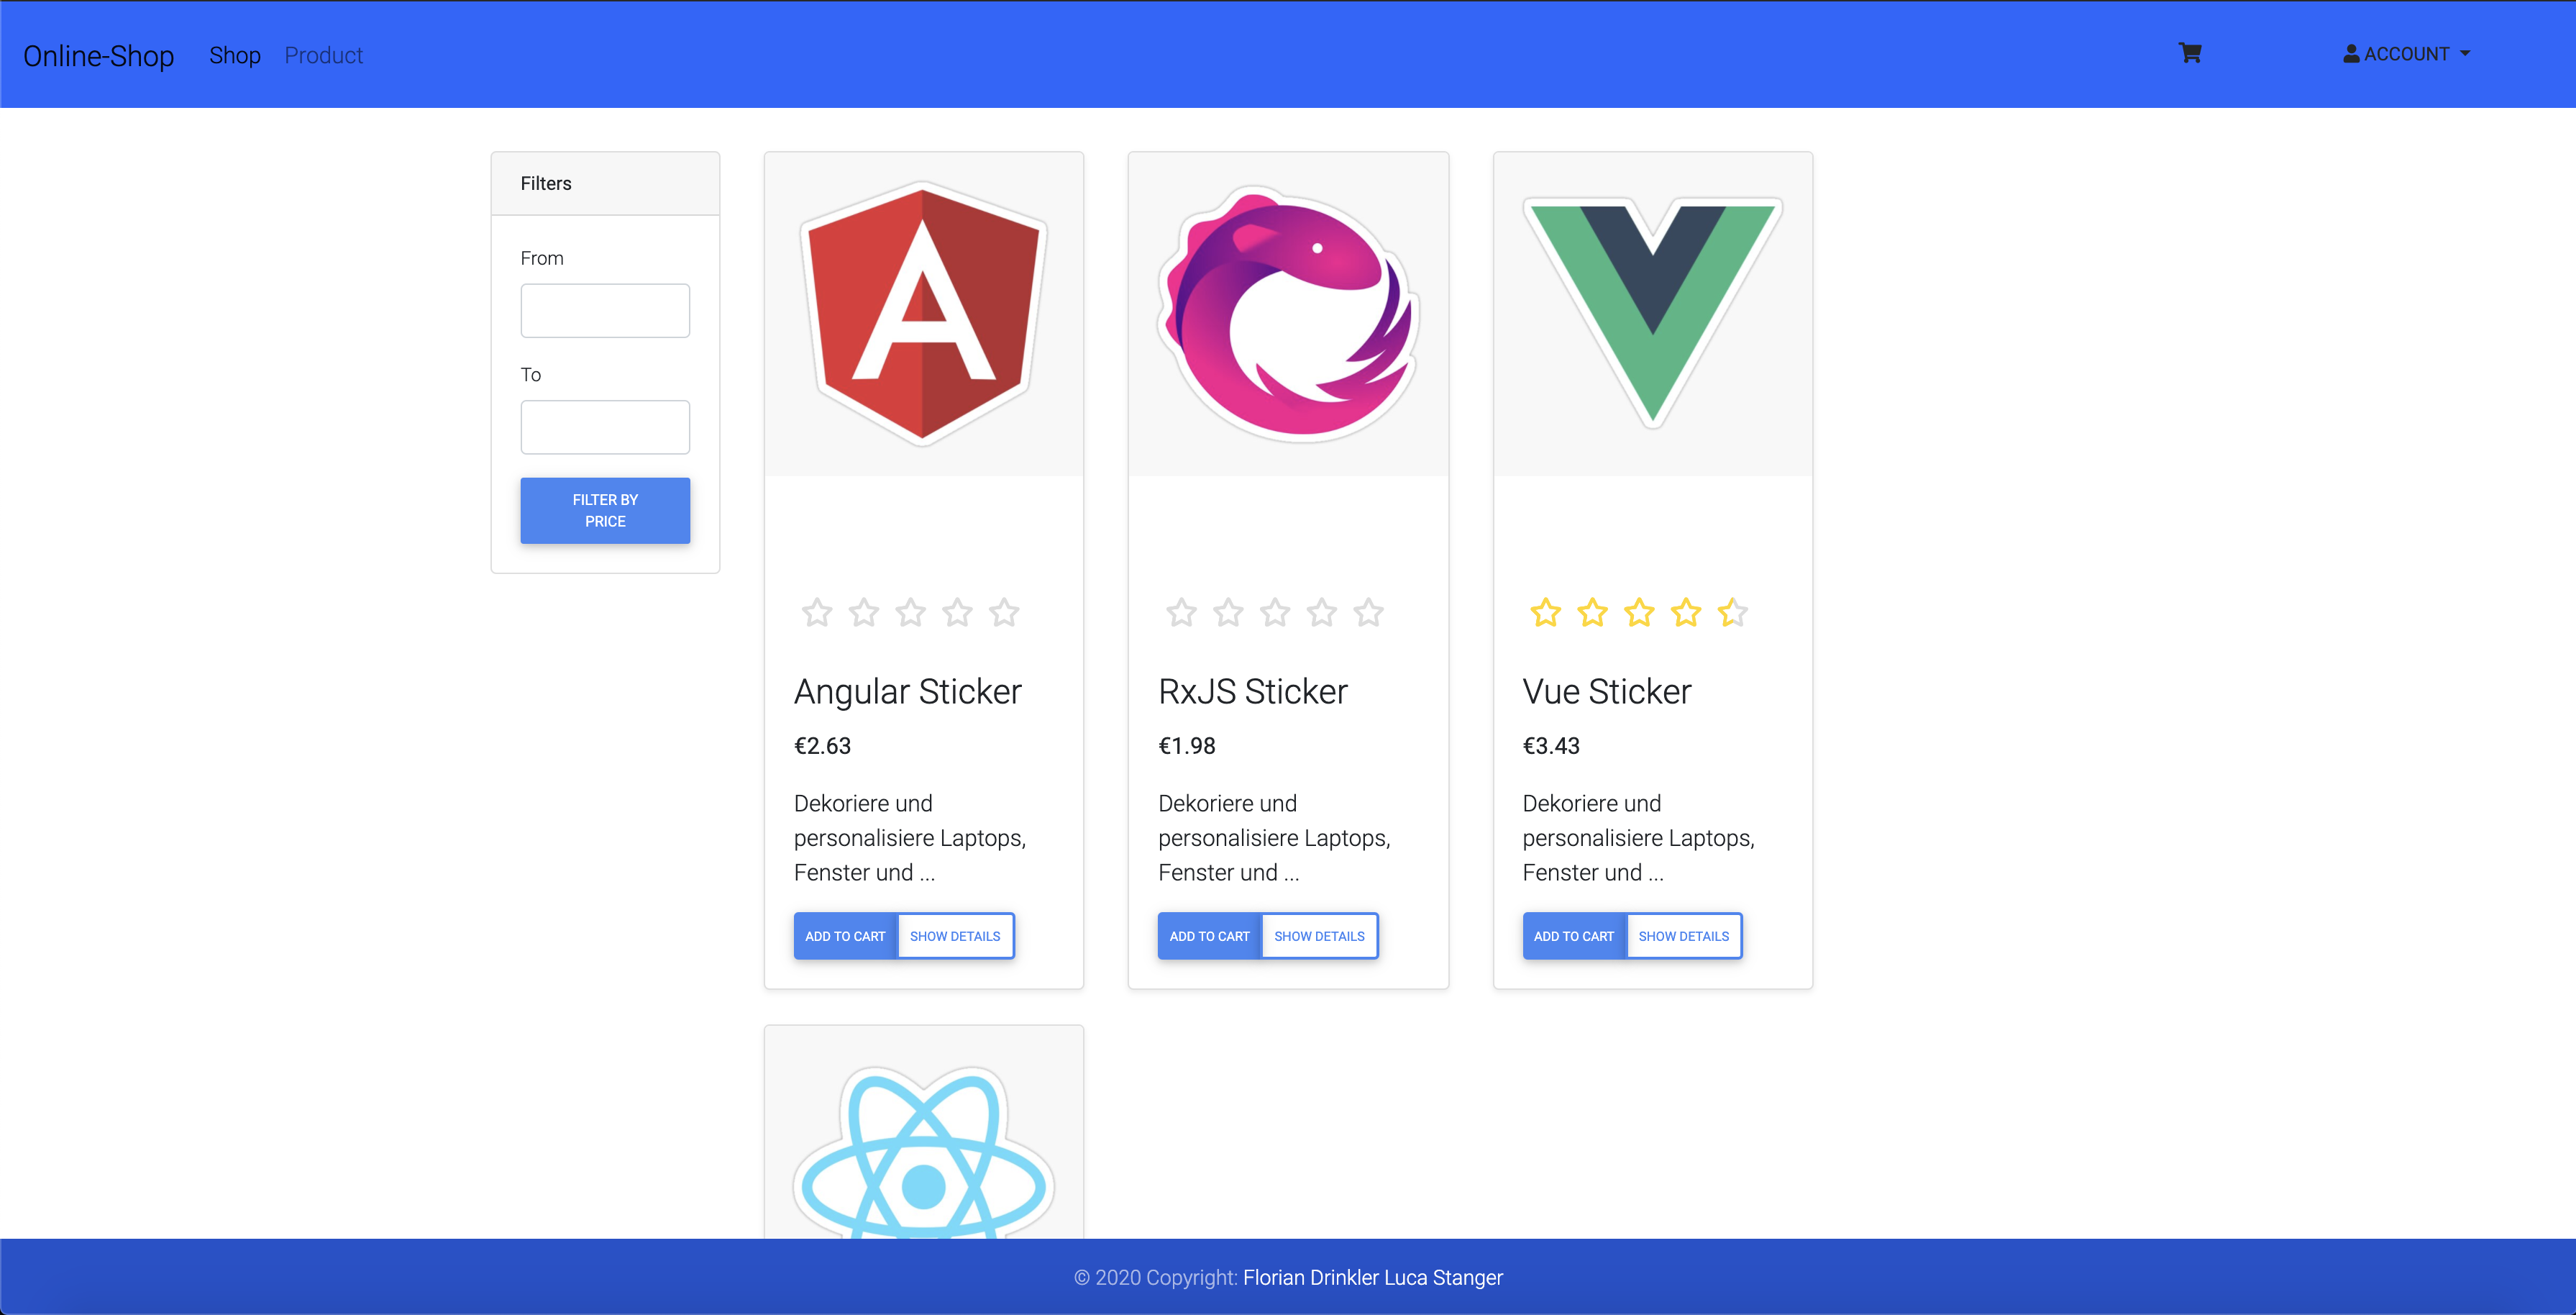
\includegraphics[width=\textwidth,height=0.6\textheight,keepaspectratio]{images/homepage.png}
 \caption{Online-Shop Startseite}
 \label{fig:homepage}
\end{figure}

\section{Produkt hinzufügen}

Um Produkte über das Frontend hinzuzufügen, kann ein Admin-Benutzer über die in der Navigations-Bar vorhandene Schaltfläche \emph{Product} die Produkt-Details hinterlegen.
Zu beachten hierbei ist, dass der eingegebene Preis durch einen Punkt getrennt wird und das Bild im Format jpg oder png hinterlegt wird.

\begin{figure}[h]
 \centering
 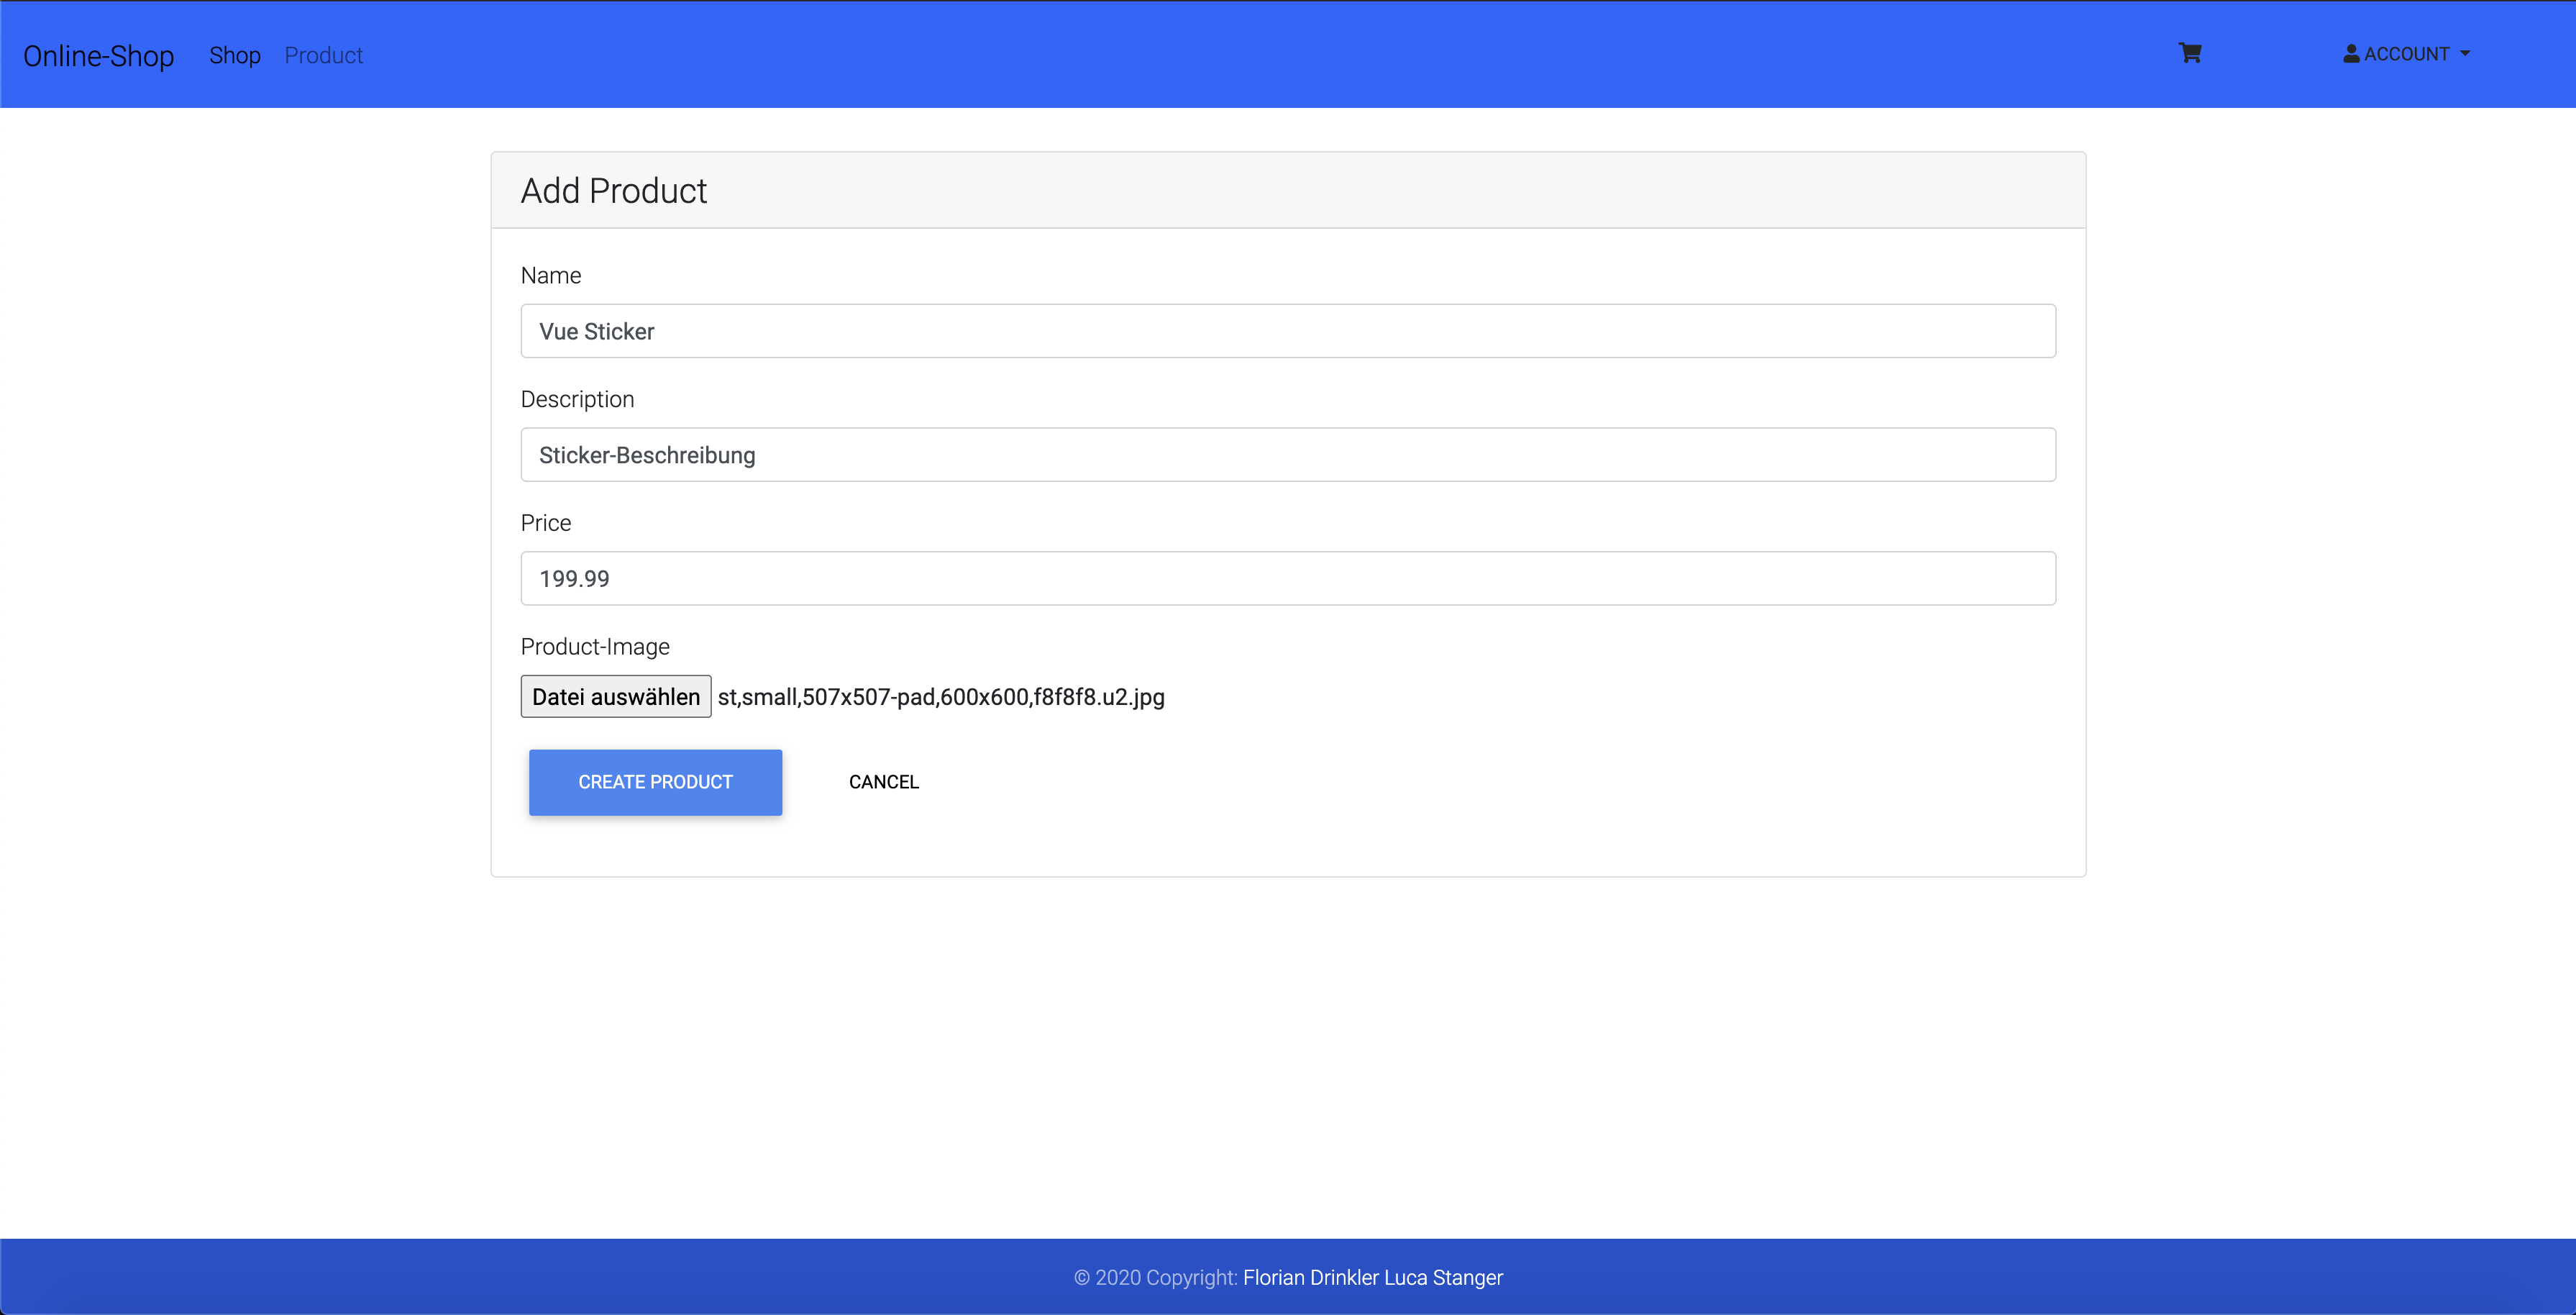
\includegraphics[width=\textwidth,height=0.6\textheight,keepaspectratio]{images/product-page.png}
 \caption{Online-Shop Startseite}
 \label{fig:product-page}
\end{figure}
\newpage
\section{Warenkorb}

Nachdem der Anwender die Produkte in den Warenkorb gelegt hat, kann dieser über die Schaltfläche \emph{Warenkorb} eine Gesamtübersicht der Produkte einsehen.

\begin{figure}[h]
 \centering
 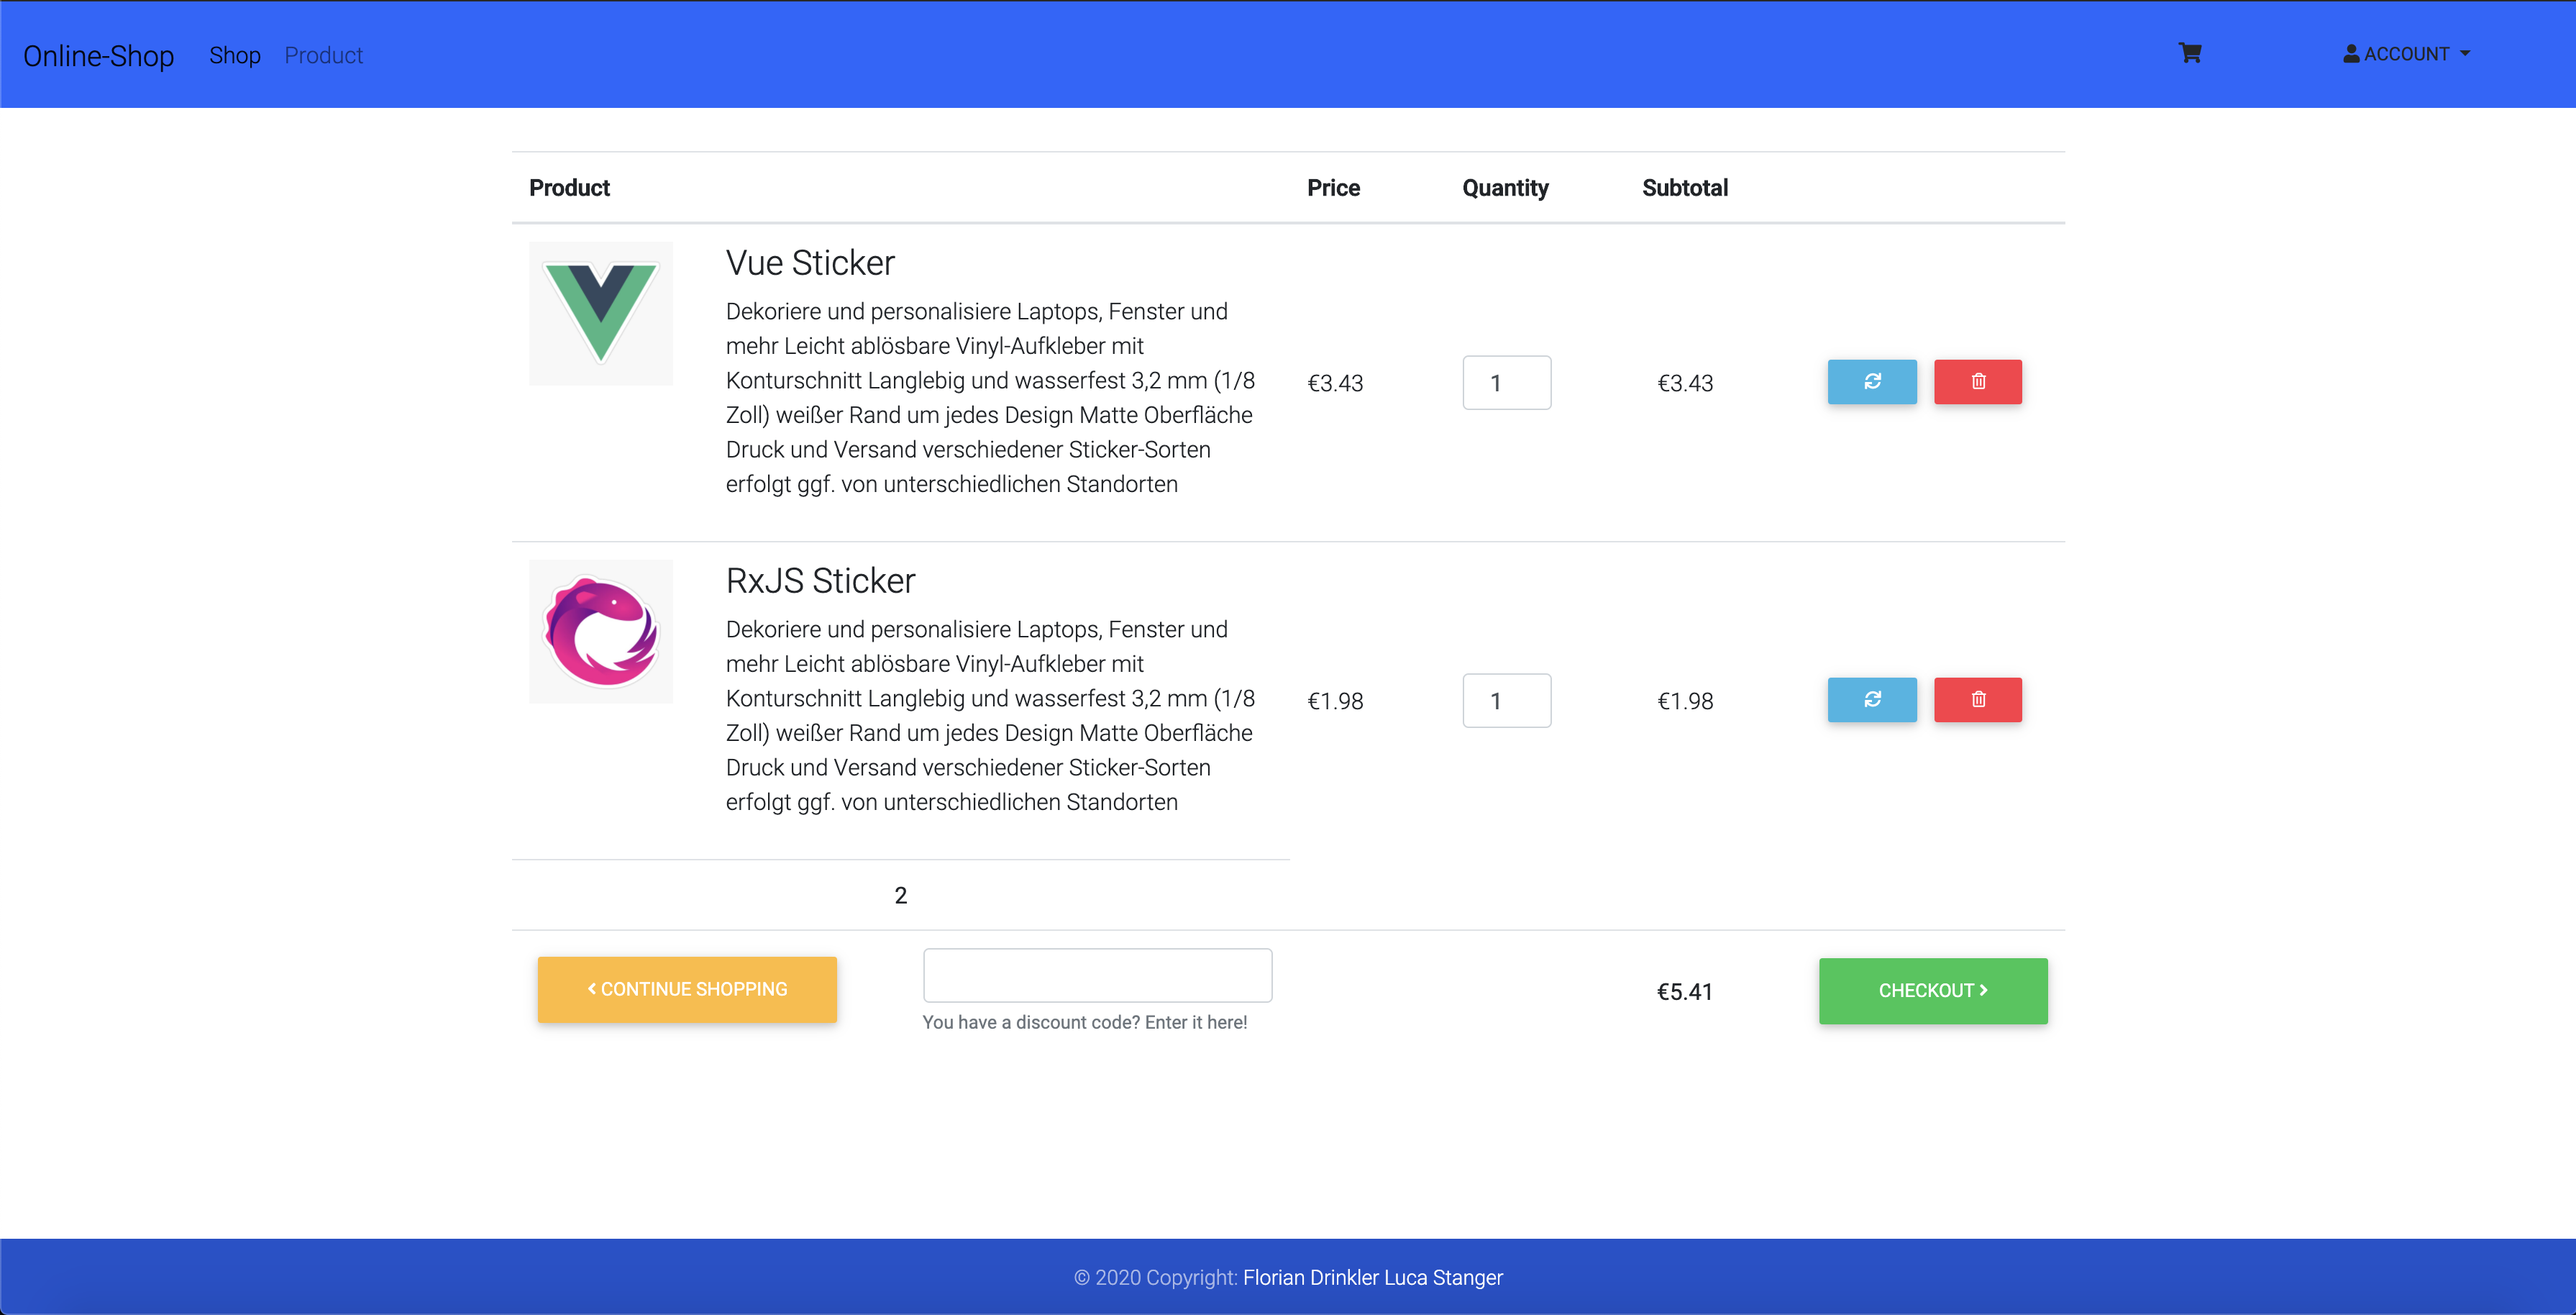
\includegraphics[width=\textwidth,height=0.6\textheight,keepaspectratio]{images/warenkorb.png}
 \caption{Online-Shop Startseite}
 \label{fig:warenkorb}
\end{figure}

Abschließend kann über den Button Checkout die Bestellung vollendet werden. Hierfür muss der Anwender seine Versanddaten eingeben. Der Warenkorb wird im Anschluss gelöscht.

Um die Software in Ihrer Funktionalität abzurunden könnte in naher Zukunft ein richtiger Checkout-Prozess implementiert werden. Da dies jedoch den Umfang des Projekts gesprengt hätte, wurde darauf verzichtet.




